\chapter{Eredmények}

A méréseket az alábbi paraméterekkel rendelkező számítógépen végeztem:
\begin{itemize}
	\item	CPU: 11th Gen Intel(R) Core(TM) i5-11300H @ 3.10GHz
	\item	GPU: NVIDIA GeForce RTX 3050Ti 
	\item	RAM: 24 GB DDR4 
	\item	OS: Windows 10 Education 22H2 
	\item	Compiler: NVCC V12.0.140
	
\end{itemize}

\section{A mérések menete}
Az algoritmusokhoz készítettem CPU és GPU kódot is. Az algoritmusok érdemi részét végig GPU-n végeztem. CPU-n a kezdeti értékeket állítottam be, különböző diagnosztikai kiíratásokat végeztem, illetve a parancssori argumentumok feldolgozását. A futásidők méréséhez az NVIDIA által készített Nsight Compute(R) programot használtam, mely képes CUDA kerneleket elemezni több szempontból is: Futási idő, Memória kihasználtsága, Grid mérete, szálanként regiszterek száma és még tovább. A program futását \ref{fig:nsight-compute}. ábrán ábrázoltam. 

\begin{figure}[ht!]
	\centering
	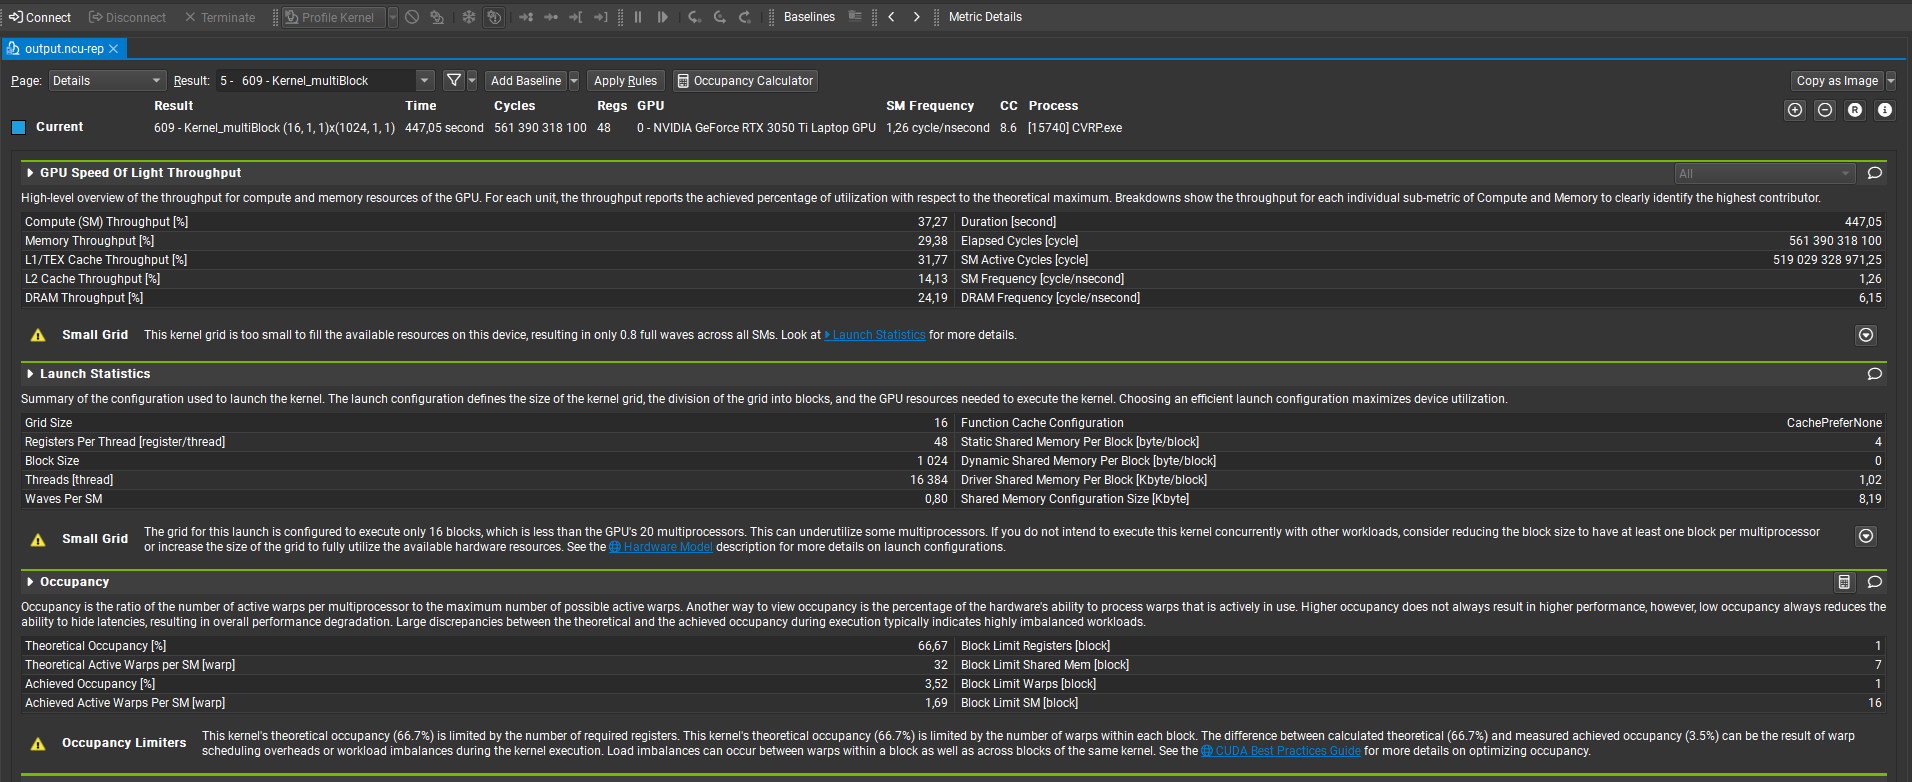
\includegraphics[width=150mm, keepaspectratio]{figures/nsight-compute.png}
	\caption{Az NVIDIA Nsight Compute program adatok széles tárházával látja el a programozót }
	\label{fig:nsight-compute}
\end{figure}

Számomra a legfontosabb a futásidő volt, ezt több különböző bemenetre és konfigurációra lemértem, majd táblázatosan összegyűjtöttem.

\section{Mérési eredmények}

\textcolor{red}{IDE VALAMI BEVEZETÉS}

\subsection{TSP első verzió}

Teszteléshez szükségem volt ismert eredményű adathalmazokra. A Floridai Állami Egyetem weboldalán \cite{TSPdataset} elérhető bárki számára több adathalmaz, különböző adatstruktúrában. Nekem a [fájlnév]\_d.txt nevű fájlok voltak hasznosak, ugyanis abban megtalálhatóak a szomszédossági mátrix költségei táblázatos alakban. Az itt található 6 adathalmazon végigfuttattam az algoritmusomat több konfigurációban. Mindig 10-szer ismételtem meg a futást, és képeztem az eredmények átlagát (számtani középpel), illetve minimumát. Nagy adathalmaz esetén hosszú a futásidő profilozó módban, ezért időmérés céljából egyszer futtattam újra ugyanazon beállításokkal. A TSP első verziójában a feromon mátrix és az élsúlyok tárolása csak double formátumban történik. Az összehasonlíthatóság érdekében egy iteráció során 20 random, és 500 tudatos hangya fut. A kezdeti feromon érték 1000, az elnyomási tényező \( \rho = 0.75 \), a jutalmazási arány 100, amely csak a 2. iterációtól érvényes (ha van).



% Size = 5
\begin{table}[ht!]
	\centering
	\begin{tabular}{|p{2cm}||p{3cm}|p{3.5cm}|p{3.5cm}|}
		\hline
		\multicolumn{4}{|c|}{FIVE : 5 csúcs, minimális út : 19, átlagos út : 24} \\
		\hline
		& Futásidő (ms) & Végeredmény átlag & Végeredmény min.\\
		\hline
		\textbf{1 rep} & & &\\
		32 ant& 7,84 & 20,2 & 19\\
		256 ant & 19,1 & 20,8 & 19\\
		1024 ant & 76,1 &	20,8 &	19\\
		\hline
		\textbf{10 rep} & & &\\
		256 ant &	137,3 & 19 &	19\\
		1024 ant & 424 &	19 &	19\\
		\hline
	\end{tabular}
	\caption{Elsőnek egy kicsi, 4 állomásból (és a 0. kiindulási pontból) álló gráfon próbáltam ki az algoritmust.}
	\label{table:TSPv1_5}
\end{table}

% Size = 15
\begin{table}[ht!]
	\centering
	\begin{tabular}{|p{2cm}||p{3cm}|p{3.5cm}|p{3.5cm}|}
		\hline
		\multicolumn{4}{|c|}{P01 : 15 csúcs, minimális út : 291, átlagos út : 662} \\
		\hline
		& Futásidő (s) & Végeredmény átlag & Végeredmény min.\\
		\hline
		\textbf{1 rep} & & &\\
		1024 ant & 0,925 & 370,2 & 291\\
		2048 ant & 1,18 & 365 & 327\\
		4096 ant & 1,20 & 359,7 & 332\\
		\hline
		\textbf{10 rep} & & &\\
		1024 ant & 11,39 & 350,4 & 291\\
		2048 ant & 11,47 & 328 & 295\\
		4096 ant & 11,59 & 336,8 & 291\\
		\hline
	\end{tabular}
	\caption{}
	\label{table:TSPv1_15}
\end{table}

A 17 vagy nála nagyobb gráfok esetében az 1 iterációs algoritmusok már olyan rosszul teljesítettek, hogy csak 10 iterációs eseteket soroltam fel a hangyák számának függvényében.

% Size = 17
\begin{table}[ht!]
	\centering
	\begin{tabular}{|p{2cm}||p{3cm}|p{3.5cm}|p{3.5cm}|}
		\hline
		\multicolumn{4}{|c|}{GR : 17 csúcs, minimális út : 2085} \\
		\hline
		& Futásidő (s) & Végeredmény átlag & Végeredmény min.\\
		\hline
		\textbf{10 rep} & & & \\
		1024 ant & 14,85 & 2391,3 & 2151\\
		2048 ant & 14,88 & 2363,4 & 2085\\
		4096 ant & 14,97 & 2279,6 & 2097\\
		8192 ant & 15,15 & 2306,4 & 2207\\
		16384 ant & 15,49 & 2250,5 & 2085\\
		\hline
	\end{tabular}
	\caption{}
	\label{table:TSPv1_17}
\end{table}

% Size = 26
\begin{table}[ht!]
	\centering
	\begin{tabular}{|p{2cm}||p{3cm}|p{3.5cm}|p{3.5cm}|}
		\hline
		\multicolumn{4}{|c|}{FRI26 : 26 csúcs, minimális út : 937, átlagos út : 2693} \\
		\hline
		& Futásidő (s) & Végeredmény átlag & Végeredmény min.\\
		\hline
		\textbf{10 rep} & & & \\
		1024 ant & 39,72 & 1386,1 & 1249\\
		2048 ant & 39,73 & 1367,1 & 1221\\
		4096 ant & 39,82 & 1227,6 & 1121\\
		8192 ant & 40,14 & 1158,7 & 1102\\
		16384 ant & 40,70 & 1132,1 & 1075\\
		\hline
	\end{tabular}
	\caption{}
	\label{table:TSPv1_26}
\end{table}

% Size = 42
\begin{table}[ht!]
	\centering
	\begin{tabular}{|p{2cm}||p{3cm}|p{3.5cm}|p{3.5cm}|}
		\hline
		\multicolumn{4}{|c|}{DANTZIG42 : 42 csúcs, minimális út : 699, átlagos út : 3110,5} \\
		\hline
		& Futásidő (s) & Végeredmény átlag & Végeredmény min.\\
		\hline
		\textbf{10 rep} & & & \\
		1024 ant & 115,41 & 1735,7 & 1554\\
		2048 ant & 113,94 & 1420 & 1252\\
		4096 ant & & 1263,8 & 1106\\
		8192 ant & & 1082,6 & 928\\
		16384 ant & 114,34 & 987,7 & 906\\
		\hline
	\end{tabular}
	\caption{}
	\label{table:TSPv1_42}
\end{table}

%%%
%

%%

% Size = 48
\begin{table}[htbp!]
	\centering
	\begin{tabular}{|p{2cm}||p{3cm}|p{3.5cm}|p{3.5cm}|}
		\hline
		\multicolumn{4}{|c|}{ATT48 : 48 csúcs, minimális út : 33523, átlagos út : 157686,9} \\
		\hline
		& Futásidő (s) & Végeredmény átlag & Végeredmény min.\\
		\hline
		\textbf{10 rep} & & & \\
		1024 ant & & &\\
		2048 ant & & &\\
		4096 ant & & &\\
		8192 ant & 152,82 & &\\
		16384 ant & 153,78 & 50197,2 & 47387 \\
		\hline
	\end{tabular}
	\caption{}
	\label{table:TSPv1_48}
\end{table}

\begin{figure}[htbp!]
	\centering
	\includegraphics[width=0.5\textwidth]{figures/TSP\_v1\_hiba.png}
	\caption{Matlabbal ábrázoltam a gráfcsúcsok számának függvényében az elméleti minimumhoz képesti átlagos hibát: TSP első verzió }
	\label{fig:TSP_v1_hiba}
\end{figure}

\subsection{TSP második (konzisztens) verzió}
Azért, hogy az előző fejezetben látott első verzióval érdemben, össze tudjam hasonlítani a mostani verziót, hasonló iterációs számokat választottam: 1 rep-en belül 20 random hangyát követ 500 tudatos hangya. Az adathalmaz is az előbbi \cite{TSPdataset} helyről származó csomag.

% Size = 15
\begin{table}[ht!]
	\centering
	\begin{tabular}{|p{2cm}||p{3cm}|p{3.5cm}|p{3.5cm}|}
		\hline
		\multicolumn{4}{|c|}{P01 : 15 csúcs, minimális út : 291, átlagos út : 662} \\
		\hline
		& Futásidő (s) & Végeredmény átlag & Végeredmény min.\\
		\hline
		\textbf{10 rep} & & &\\
		1024 ant & 2,69 & 320  & 307\\
		2048 ant & 2,82 & 307,6 & 291\\
		4096 ant & 2,97 & 305,4 & 291\\
		8192 ant & 3,19 & 300,2 & 291\\
		12288 ant & 3,50 & 296,4 & 291\\
		16384 ant & 3,73 & 294,6 & 291\\
		20480 ant & 3,92 & 295,4 & 291\\
		\hline
		\textbf{30 rep} & & &\\
		1024 ant & 8,05 & 301,6 & 291\\
		\hline
	\end{tabular}
	\caption{}
	\label{table:TSPv2_15}
\end{table}

% Size = 17
\begin{table}[ht!]
	\centering
	\begin{tabular}{|p{2cm}||p{3cm}|p{3.5cm}|p{3.5cm}|}
		\hline
		\multicolumn{4}{|c|}{GR : 17 csúcs, minimális út : 2085} \\
		\hline
		& Futásidő (s) & Végeredmény átlag & Végeredmény min.\\
		\hline
		\textbf{10 rep} & & & \\
		1024 ant & 3,54 & 2246 & 2094\\
		2048 ant & 3,69 & 2237,7 & 2207\\
		4096 ant & 3,69 & 2196,5 & 2142\\
		8192 ant & 3,89 & 2211,5 & 2170\\
		16384 ant & 4,37 & 2179,2 & 2129\\
		20480 ant &  &  & \\
		\hline
	\end{tabular}
	\caption{}
	\label{table:TSPv2_17}
\end{table}

% Size = 26
\begin{table}[ht!]
	\centering
	\begin{tabular}{|p{2cm}||p{3cm}|p{3.5cm}|p{3.5cm}|}
		\hline
		\multicolumn{4}{|c|}{FRI26 : 26 csúcs, minimális út : 937, átlagos út : 2693} \\
		\hline
		& Futásidő (s) & Végeredmény átlag & Végeredmény min.\\
		\hline
		\textbf{10 rep} & & & \\
		1024 ant & 9,00 & 1393 & 1347\\
		2048 ant & 9,23 & 1363,1 & 1288\\
		4096 ant & 9,43 & 1215,3 & 1163\\
		8192 ant & 9,72 & 1136,9 & 1055\\
		16384 ant & 10,82 & 1104,9 & 1007\\
		20480 ant &  &  & \\
		\hline
	\end{tabular}
	\caption{}
	\label{table:TSPv2_26}
\end{table}

% Size = 42
\begin{table}[ht!]
	\centering
	\begin{tabular}{|p{2cm}||p{3cm}|p{3.5cm}|p{3.5cm}|}
		\hline
		\multicolumn{4}{|c|}{DANTZIG42 : 42 csúcs, minimális út : 699, átlagos út : 3110,5} \\
		\hline
		& Futásidő (s) & Végeredmény átlag & Végeredmény min.\\
		\hline
		\textbf{10 rep} & & & \\
		1024 ant & 26,19 & 1601,3 & 1018\\
		2048 ant & 26,61 & 1488,4 & 1319\\
		4096 ant & 27,02 & 1286,7 & 1168\\
		8192 ant & 27,57 & 1118,3 & 1004\\
		16384 ant &  & 1014,7 & 909\\
		20480 ant &  &  & \\
		\hline
	\end{tabular}
	\caption{}
	\label{table:TSPv2_42}
\end{table}

%%%
%

%%

% Size = 48
\begin{table}[htbp!]
	\centering
	\begin{tabular}{|p{2cm}||p{3cm}|p{3.5cm}|p{3.5cm}|}
		\hline
		\multicolumn{4}{|c|}{ATT48 : 48 csúcs, minimális út : 33523, átlagos út : 157686,9} \\
		\hline
		& Futásidő (s) & Végeredmény átlag & Végeredmény min.\\
		\hline
		\textbf{10 rep} & & & \\
		1024 ant & 38,12& 84660,7& 67541 \\
		2048 ant & 38,63 & 72522,8 & 64969 \\
		4096 ant &39,14&62808,6&53395 \\
		8192 ant & 39,69 & 59604,8 & 52514\\
		16384 ant & 41,56&48618,2&46227 \\
		20480 ant & 124,72 & 49879,9 & 45836\\
		\hline
	\end{tabular}
	\caption{}
	\label{table:TSPv2_48}
\end{table}

% Empty
\begin{table}[ht!]
	\centering
	\begin{tabular}{|p{2cm}||p{3cm}|p{3.5cm}|p{3.5cm}|}
		\hline
		\multicolumn{4}{|c|}{} \\
		\hline
		& Futásidő (s) & Végeredmény átlag & Végeredmény min.\\
		\hline
		\textbf{10 rep} & \\
		1024 ant & \\
		2048 ant & \\
		4096 ant & \\
		8192 ant & \\
		16384 ant & \\
		20480 ant & \\
		\hline
	\end{tabular}
	\caption{}
	\label{table:TSPv2_empty}
\end{table}

\subsection{VRP}
A VRP-hez eleinte nem értettem, hogy miért nem találtam külön adathalmazt. Később megértettem, hogy mivel nincs megadva egyéb feltétel, (általában) teljesen mindegy, hogy hány járművet használhat az algoritmus, a legjobban akkor fog járni, ha az összes állomást ugyanazon járművel járja végig.

\subsection{CVRP}
Az első olyan algoritmus, amely feltételes útvonaltervezést igényel, a Kapacitásos jármű útvonaltervezési feladat. Adathalmazt a \textcolor{red}{HIÁNYZIK} helyről szedtem.
Az iterációk az előzőeknél látottakkal megegyezőek: 1 rep-en belül 20 random hangyát követ 500 tudatos hangya.

% Size = 17
\begin{table}[ht!]
	\centering
	\begin{tabular}{|p{2cm}||p{3cm}|p{3.5cm}|p{3.5cm}|}
		
		\hline
		& Futásidő (s) & Végeredmény átlag & Végeredmény min.\\
		\hline
		\textbf{10 rep} & \\
		1024 ant & \\
		2048 ant & \\
		4096 ant & \\
		8192 ant & \\
		16384 ant & \\
		20480 ant & \\
		\hline
	\end{tabular}
	\caption{}
	\label{table:TSPv2_empty}
\end{table}

% Size = 17
\begin{table}[ht!]
	\centering
	\begin{tabular}{|p{2cm}||p{3cm}|p{3.5cm}|p{3.5cm}|}
		
		\hline
		& Futásidő (s) & Végeredmény átlag & Végeredmény min.\\
		\hline
		\textbf{10 rep} & \\
		1024 ant & \\
		2048 ant & \\
		4096 ant & \\
		8192 ant & \\
		16384 ant & \\
		20480 ant & \\
		\hline
	\end{tabular}
	\caption{}
	\label{table:CVRP_empty}
\end{table}


\section{Eredmények értékelése}

szép grafikonok plusz rizsa: több szál = lassabb, de jobb eredmény